\documentclass[a4paper,man,natbib,floatsintext,12pt]{apa7}

\usepackage[english]{babel} %character and hyphenation rules specific to the language you choose
%\usepackage[utf8x]{inputenc}
\usepackage{graphicx}
\usepackage{color}
\usepackage{tikz}
\usepackage{amsmath}
\usepackage{blindtext}
\usepackage{tabularx} %great for APA-style Tables
\usepackage{siunitx} % Required for good table alignmen
\sisetup{
  round-mode          = places, % Rounds numbers
  round-precision     = 2, % to 2 places
}
\usepackage{texlive-bibtexextra}
\usepackage{multirow}
\usepackage{booktabs}
\usepackage{wrapfig}
\usetikzlibrary{shapes,decorations,arrows,calc,arrows.meta,fit,positioning}
\tikzset{
    -Latex,auto,node distance =1 cm and 1 cm,semithick,
    latent/.style ={ellipse, draw, minimum width = 0.7 cm},
    observed/.style ={rectangle, draw},
    bidirected/.style={Latex-Latex,dashed},
    el/.style = {inner sep=2pt, align=left, sloped}
}
\newcommand{\sigFtest}[4]{\textit{F}(#1,#2) = #3, \textit{p}$<$#4}
\newcommand{\nonsigFtest}[3]{\textit{F}(#1,#2) = #3, \textit{p}$>$.05}

\title{Confirming the External Validity of Cognitive Control via ERP Measures }
\shorttitle{Testing for Sam's Thesis}
\author{Samantha J. Kline}
\affiliation{College of William \& Mary}
\journal{Thesis Manuscript}
\abstract{The abstract of my thesis will go here. It will include details from the intro, methods, results and discussion.}
\keywords{Cognitive Control, Event-Related Potential, Alcohol}
\authornote{These are the notes that I will put in my thesis}
\leftheader{Alternate page header in man mode}

%-------------- END PREAMBLE  -------------------


\begin{document}

\maketitle  %Insert my APA style title page

\section{Introduction}

Cognitive control is thought to support adaptive behavior by overcoming automatic, impulsive responses. Longstanding theoretical models propose cognitive moderates the relationship between automatic impulses and later behavior \citep{diamond13}. This is also assumed in neural measures, with the P300 event-related potential (ERP) often used to quantify cognitive control. However, no studies have directly tested this moderation. What is also unclear is how this assumed relationship is altered in features associated with deteriorated cognitive control, such as among impulsive individuals and those who engage in heavy or uncontrolled alcohol use. Heavy alcohol use during late adolescence (i.e., college-age) can have deleterious effects on neurological development as critical brain regions are undergoing maturation. This includes the prefrontal cortex, which is implicated in cognitive control function. Rates of alcohol use continue to remain a pervasive issue in the United States. 49.6 \% (16.9 million) of Americans aged reported alcohol use in the last month. This is attributable to many sources, but namely due to the belief that drinking is a core aspect of the college experience \citep{tan12}. Heavy drinking in college is cause for concern due to the neuro-developmental implications. The typical college-age (18-24 years) aligns with the late adolescent period, where essential brain regions are undergoing maturation. The prefrontal cortex (PFC) is just one example of this. Impaired PFC is linked to impulsive behavior such as experimenting with alcohol and other drugs and the PFC is considered is a critical area for cognitive control function. It is also broadly theorized that correlates of cognitive control behave differently among heavy drinkers. However, this model has yet to be tested in this manner. Cognitive control functions as an umbrella of several mechanisms including response inhibition and interference control. Cognitive control is typically measured using tasks that elicit response conflict, including Simon (response inhibition) and Flanker (interference control) tasks. Simon conflict reflects the automatic tendency to respond with the hand ipsilateral to a stimulus regardless of the correct response. Flanker conflict occurs when irrelevant flanking stimuli indicate a response unrelated to the target stimulus. Few studies have examined how different cognitive control mechanisms interact and no studies have explored this interaction in the context of clinical features such as hazardous alcohol use or impulsivity. ERPs reflecting cognitive control and early response preparation will be compared to task performance (reaction time, accuracy) to test the hypotheses that (1) cognitive control (Via P3 ERP amplitude) moderates prepotent response activation and behavior, and (2) because cognitive control is reduced in high binge drinking and impulsivity, the moderation is weakened, leading to a strengthened relationship between impulsive response activation and unsuccessful inhibition (poor task performance). 

\section{Method}

\subsection{Participants}
\begin{itemize}
	\item 120 college-age participants will be recruited via SONA to participate in this study.
	\item Participants will be compensated for their time with course credit. 
	\item Anyone who reports history of seizure disorder, a neurodegenerative disease or past year concussion will not be permitted to participate. 
	\item Written informed consent will be obtained before any data is collected and the study has full IRB approval.
\end{itemize}
\subsection{Materials and Procedure}
\begin{itemize}
	\item After informed consent is given, participants will complete a demographics survey. Additionally, they will be asked to complete the Alcohol Use Disorders Identification Test (AUDIT) and Brief Impulsive Behavior Short Scale (I-8).
	\item All forms will be completed on PsyToolKit. 
	\item After the EEG set up is complete, participants will begin a combined Simon-Flanker task on PsychoPy. 
	\item The EEG data will be recorded continuously to record conflict processing activity throughout the task.
	\item The task consists of a total of 480 trials and total procedures take about 1 hour on average.
\end{itemize}

\section{Results}
This is the data analysis plan for this study. This section also includes figures from my first year project that can outline the current direction of my thesis. 
\begin{itemize}
	\item Once data collection is complete, the data will be cleaned and processed using standard protocol. Data will be processed in EEGLab via MATLAB. Difference waveforms will be calculated by subtracting the conflict conditions (SCFI, SIFC and SIFI) from SCFC.
	\item These difference waveforms will be used to extract pure conflict processing activity and remove other irrelevant mental processes. 
	\item Planned statistical analyses include repeated-measures ANOVA for the different variables including LRP, P3 and reaction time. Additionally, linear mixed models will be used to test the interactions between P3 and LRP across different conflicts and conditions. Analyses will also incorporate AUDIT and I-8 scores to examine differences between heavy drinkers and highly impulsive individuals from healthy controls. 
	\item The main analysis may simplify by focusing on Equal condition and SIFI, but exploratory analyses (TBD) will determine how AUDIT and I-8 scores relate to the different conflicts and conditions. 
	\item The base for my thesis will be an expanded version of the theoretical model of my FYP.
\end{itemize}
\begin{figure}[ht!]
\centering
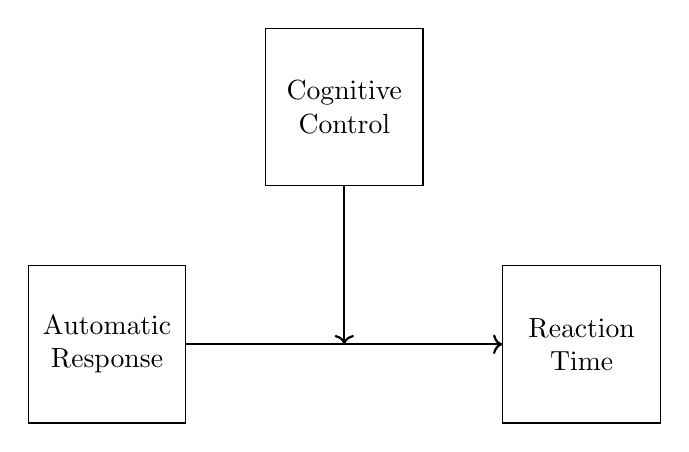
\begin{tikzpicture}
\usetikzlibrary{positioning}
\node [draw, align=center, minimum width=2cm, minimum height=2cm, inner sep=2pt] (CC) at (0,0) {Cognitive\\ Control};
\node [draw, align=center, minimum width=2cm, minimum height=2cm, inner sep=2pt] (RT) [below right=of CC] {Reaction\\ Time};
\node [draw, align=center, minimum width=2cm, minimum height=2cm, inner sep=2pt] (LRP) [below left=of CC] {Automatic \\ Response};
\path[->,thick](LRP)edge(RT);
\path (LRP) -- (RT) coordinate[midway] (midpoint);
\draw [->,thick](CC) -- (midpoint);
\end{tikzpicture}
\caption{Here is the theoretical model that my thesis will be expanding.}
\label{fig:FYP} 
\end{figure}

\begin{figure}[htbp] 
\centering
\includegraphics[width=0.8\textwidth]{totalfigs_copy}
\caption{Here are some figures for my P3b and LRP data}
\label{fig:ERPs}
\end{figure}

\begin{table}[h!]
\centering
\caption{\label{tab:RTmeans}Reaction times for different Simon-Flanker conflict and PC effect conditons.}
\begin{tabular}{l l c c c}
 \toprule
                          &              & \multicolumn{3}{c}{Condition, seconds}\\
  \cmidrule{3-5}
                          &              & {Equal}           & {Incongruent}           & {Congruent}\\
  \cmidrule{3-5}
  \multirow{ 4}{*}{Conflict} & SCFC &     0.595    &      0.603     &      0.585     \\
                          & SCFI      &     0.654      &      0.671     &      0.639   \\
                          & SIFC     &     0.624     &     0.621     &     0.641     \\
                          & SIFI     &      0.712    &     0.703     &     0.716    \\
  \bottomrule
 \end{tabular}
\end{table}


\section{Discussion}
Once data collection and statistical analyses are complete, the results will be discussed here (see Table~\ref{tab:RTmeans}). 

These results will advance the field in several ways. First, it will expand the current theoretical perspective regarding cognitive control using an approach that accounts for the different cognitive control mechanisms. Additionally, the outcomes of this study may inform of cognitive deficits among heavy drinkers prior to progression to alcohol use disorder. The use of EEG is especially important for that feature. Incorporating impulsivity is another approach to testing the external validity of this cognitive control model using a trait common in many clinical disorders. In the long-run, this study will hopefully advance the current understanding of both the neural bases of cognitive control and how alcohol use can alter this mechanism. This information can be used to inform the general public of the risks associated with alcohol use specifically during late adolescence. ERPs from this study can also be used as biomarkers for increased sensitivity for later alcohol use disorder. Overall this study will importantly clarify neural components of cognitive control as it fits with the current theoretical approach and expand the field's understanding of adolescent alcohol use and impulsive behaviors. 

This is a figure of the ERP scalp map. I included this as an additional figure to show how the many ways to convey EEG data in a paper. 

\begin{wrapfigure}{l}{0.4\textwidth}     \centering       
\includegraphics[width=0.25\textwidth]{scalpfig_copy}
\caption{\label{fig:latbrain} This figure was taken at 600 ms post-stimulus presentation .}
\end{wrapfigure}

Figure~\ref{fig:ERPs} This is another link to the sample data from my FYP.


\bibliography{references}

\end{document}
https://www.overleaf.com/project/64ef8e5b3faa92d4248ddcf9